\documentclass[
	classe=$2^{de}$,
	headerTitle=Activité\space Chapitre\space 3,
	landscape,
	twocolumn
]{exercice}

\title{Translations}

\begin{document}

\newcommand{\Activite}{
	\maketitle

	\begin{enumerate}
		\item On a ci-dessous une figure. Deux points d'une nouvelle figure on déjà été placés : la compléter.

		      \begin{tikzpicture}
			      \draw
			      (0,0) node[above left] {A}
			      -- ++(1,-1) node[below] {B}
			      -- ++(2,0) node[below] {C}
			      -- ++(-2,2) node[right] {D}
			      -- ++(0,2) node[above] {E}
			      -- ++(-2,0) node[above] {F}
			      -- ++(2,-2)
			      -- ++(-2,-2) node[below] {H}
			      -- ++(0,2) node[left] {I}
			      -- ++(1,1) node[above right] {J};

			      \draw
			      (6,-1) node[above left] {A'}
			      -- ++(1,-1) node[below] {B'}
			      \correctionOr{-- ++(2,0) node[below] {C'}
				      -- ++(-2,2) node[right] {D'}
				      -- ++(0,2) node[above] {E'}
				      -- ++(-2,0) node[above] {F'}
				      -- ++(2,-2)
				      -- ++(-2,-2) node[below] {H'}
				      -- ++(0,2) node[left] {I'}
				      -- ++(1,1) node[above right] {J'}}{};
			      % \node at (9,0) {\phantom{A}};
		      \end{tikzpicture}

		\item Comment appelle-t'on le passage de la première figure à la deuxième ?
		      \correction{Une translation.}
		\item Pour chaque situation ci-dessous, s'agit-il d'une situation de translation ?
		      \begin{multicols}{2}
			      \begin{enumerate}
				      \item 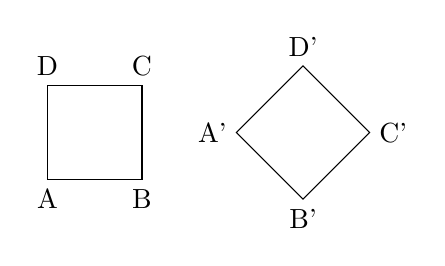
\begin{tikzpicture}[scale=0.6]
					            \newcommand{\sqrtTwo}{1.41}
					            \draw (0,0) node[below] {A}
					            -- ++(2,0) node[below] {B}
					            -- ++(0,2) node[above] {C}
					            -- ++(-2,0) node[above] {D} -- cycle;
					            \draw (4,1) node[left] {A'}
					            -- ++(\sqrtTwo,-\sqrtTwo) node[below] {B'}
					            -- ++(\sqrtTwo,\sqrtTwo) node[right] {C'}
					            -- ++(-\sqrtTwo,\sqrtTwo) node[above] {D'} -- cycle;
				            \end{tikzpicture}
				      \item 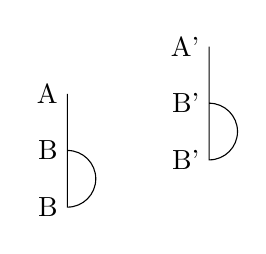
\begin{tikzpicture}[scale=0.6]
					            \draw (0,0) node[left] {A}
					            -- ++(0,-2.4) node[left] {B}
					            arc (-90:90:0.6) node[left] {B};
					            \draw (3,1) node[left] {A'}
					            -- ++(0,-2.4) node[left] {B'}
					            arc (-90:90:0.6) node[left] {B'};
				            \end{tikzpicture}
				      \item 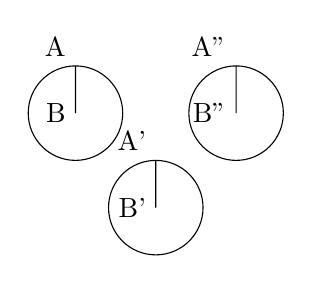
\begin{tikzpicture}[scale=0.6]
					            \draw (0,0) node[above left] {A} -- ++(0,-1) node[left] {B} circle (1);
					            \draw (1.7,-2) node[above left] {A'} -- ++(0,-1) node[left] {B'} circle (1);
					            \draw (3.4,0) node[above left] {A''} -- ++(0,-1) node[left] {B''} circle (1);
				            \end{tikzpicture}
				      \item 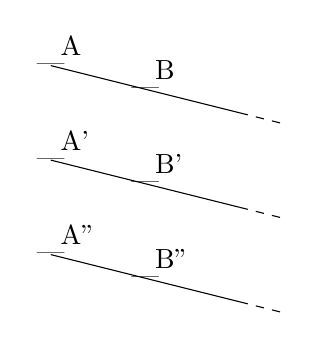
\begin{tikzpicture}[scale=0.6]
					            \draw (0,0) node{|} node[above right] {A}
					            -- ++(2,-0.5) node{|} node[above right] {B} -- ++(2,-0.5);
					            \draw[dashed] (0,0) ++(4,-1) -- ++(1,-0.25);
					            \draw (0,-2) node{|} node[above right] {A'}
					            -- ++(2,-0.5) node{|} node[above right] {B'} -- ++(2,-0.5);
					            \draw[dashed] (0,-2) ++(4,-1) -- ++(1,-0.25);
					            \draw (0,-4) node{|} node[above right] {A''}
					            -- ++(2,-0.5) node{|} node[above right] {B''} -- ++(2,-0.5);
					            \draw[dashed] (0,-4) ++(4,-1) -- ++(1,-0.25);
				            \end{tikzpicture}
			      \end{enumerate}
		      \end{multicols}
	\end{enumerate}
}

\Activite

\newpage

\Activite

\end{document}